%!TEX root = ../dissertation.tex

\begin{savequote}[75mm]
What is different between many-body localization and the atoms in this table?
\qauthor{Professor Adam Kaufman}
\end{savequote}

%\begin{savequote}[75mm]
%So what is quantum many-body about this?
%\qauthor{-Professor Misha Lukin}
%\end{savequote}
%
%\begin{savequote}[75mm]
%Re: Aren't we all?
%\qauthor{-Dominik Wild}
%\end{savequote}

\chapter{Correlation dynamics \newline in many-body localization}
\label{sec:ch5}

In the previous section, the generic behavior for a pure quantum state of an interacting many-body system was presented in the context of the eigenstate thermalization hypothesis (ETH). This hypothesis predicts that when such a system is brought far from equilibrium, it will locally equilibrate to the prediction of a thermal ensemble while remaining in a pure quantum state. This prediction relies on the fact that the eigenstates themselves are chaotic and are in a superposition of all (many) of the available microstates that satisfy global thermodynamic constraints \cite{Deutsch1991,Srednicki1994,Rigol2008,Neill2016,Kaufman2016}. A consequence of this eigenstate property is that local information about the initial state is scrambled and transferred into non-local correlations that are only accessible through a few special global observables.

A narrower class of systems that do not exhibit such chaotic eigenstates are known as integrable systems. They harbor an extensive set of locally conserved quantities that prevent the ergodic phase space exploration required for the ETH and classical statistical ensembles\cite{DAlessio2016}. In the case of non-interacting systems, the addition of local disorder was shown to create all eigenstates of the system to be constructed out of localized orbitals\cite{Anderson1958,Schwartz2007,Billy2008,Roati2008,Lahini2008,Deissler2010,Gadway2011,Kondov2011,Jendrzejewski2012,DErrico2008}. These localized orbitals become the extensive set of locally conserved quantities that makes the system an integrable one. The addition of inter-particle interactions was thought to generically lead to the breaking of this integrability by allowing for hybridization between these localized orbitals return the system to a thermalizing one.\footnote{In a classical sense, the thought would be that inter-particle interactions would allow for ergodic exploration of phase space since interactions would allow the particles to exchange energy and eventually equilibrate in their potential landscape -- although it may take a very long time.} However, as speculated by \emph{Anderson}\cite{Anderson1958} it turns out that even in the case of relatively strong interactions, the addition of sufficiently strong disorder can make the system integrable and inhibit thermalization. This paradigmatic example of such an integrable, many-body system is known as many-body localization (MBL) \cite{Nandkishore2015,Anderson1958,Kondov2015,Semeghini2015,Gornyi2005,Basko2006,Oganesyan2007,Vosk2015}. Since the system does not thermalize, its dynamics to not lead to relaxation of an initial state through the scrambling of all local information throughout the remaining system -- using it as a functional bath like. Such an onset of localization has previously been probed by a lack of thermalization (i.e. lack of ergodic space exploration) in a system of interacting particles\cite{Schreiber2015,Smith2016,Choi2016}.

We will explore many-body localization for a Bose-Hubbard system where on-site disorder is used to suppress the transport of particles in the system and, in doing so, preserves a memory of the initial state that signals a lack of ergodic exploration of the system. We observe this onset of integrability at a finite disorder strength and can independently probe the localization of particles. Importantly, we additionally verify the system is an interacting, many-bodied one: even though particle transport has been suppressed, the interactions in the system continue the spread of non-local correlations throughout the system \cite{Lukin2019}. These non-local correlations exist within the manifold of available states that are limited by particle localization. These dynamics are considered to be the hallmark of MBL are absent for a localized, non-interacting system. These characteristics are due to the change in the behavior of nearly all the eigenstates in the system and realize a non-equilibrium phase of the quantum system. It is additionally the only known robust form for breaking ergodicity and the application of the ETH in an interacting system \cite{Nandkishore2015}. Unlike other integrable, interacting systems, MBL is not fine tuned and small perturbations applied to the system do not destroy its integrability.

%-- the persistence of coherent many-body dyancmis 

\section{Localization in the interacting Aubry-Andr\'e model}
\label{sec:ch5AAM}

In our experiments, we study MBL in the interacting Aubry-Andr\'e model for bosons in a one-dimensional lattice \cite{Huse2014,Aubry1980}. This model is described by the Hamiltonian:

\begin{equation}
\label{eqn:aaham}
\hat{H} = -J\sum_i \left ( \hat{a}_i^\dagger \hat{a}_{i+1} + h.c. \right ) + \frac{U}{2} \sum_i \hat{n}_i \left (\hat{n}_i - 1 \right ) + W \sum_i h_i \hat{n}_i
\end{equation}

where the on-site potential offsets are derived from an incommensurate (quasi-periodic) distribution described by $h_i = \cos{\left ( 2 \pi i \beta + \phi \right )} $ with a spatial frequency of $\beta \approx 1.618$ sites${^{-1}}$ as an approximation of the golden ratio ($\beta_{GR} = \frac{\sqrt{5}+1}{2}$). \footnote{This is often called ``quasi-periodic disorder" to describe this distribution of offsets. While the function is, of course, exactly periodic, its ratio is incommensurate with the physics lattice periodicity and hence any given on-site offset will never be resampled in the system on any length scale. This intrinsic prevention of resampling adds inherent structure to the system that lead to spatial correlations that should discourage one from thinking of it as truly ``disorder" as investigated for the Anderson localization problem. However, for a practical comparison of both localizing phenomena, it is the on-site potential that leads to localization and hence inherints the common terminology of ``disorder".} The phase offset $\phi$ is changed for different measurements such that the results are characteristic of a general phenomena and not descriptive of a single potential realization. We use the DMD discussed earlier in this thesis (\S \ref{sec:ch2DMD}) to project this on-site potential offsets onto the bare lattice with some overall scaling strength represented by W in (\ref{eqn:aaham}). 

\begin{figure}[t!]
		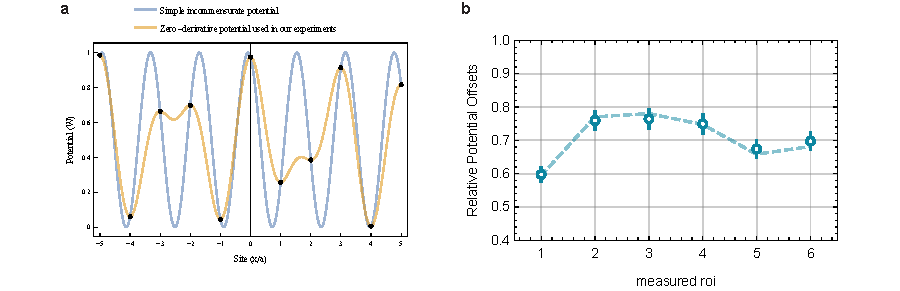
\includegraphics[width=\columnwidth]{figures/ch5/combo_disorder.pdf} 
		\caption{\textbf{Applied on-site potential and calibration. a)} The theoretically prescribed quasi-periodic potential (blue) and the physically implemented potential (yellow) are plotted together to show that they sample the same points at every physical lattice site. Importantly, the implemented potential has extrema at at each lattice site which is locally quadratic and is therefore insensitive to shaking at first order. \textbf{b)} The applied DMD potential was calibrated by a method mentioned in \S \ref{sec:DMDpotCal} where we find excellent agreement between the predicted relative potential offsets and the measured ones. All error bars are the s.e.m.}
		\label{fig:comboDisorder}	
\end{figure}

Observing the slow coherent dynamics in the many-body localized system additionally requires the quantum system remains well isolated from the environment for long experimental times. Since the optical path for the optical lattice and the projected on-site potentials are not the same, any residual physical vibrations on the optical table or air currents in the optical path will result in relative shaking between the two potentials. In the bare formulation of $h_i$, as written above, some sites additionally have a non-zero potential gradient ($d h(x)/dx \rvert_{x=x_i} \neq 0$). Any shaking of the optical path will realize this on-site potential gradient into an on-site potential modulation $h_i(t)$ that prevents the system from being time-independent; effectively, this weakly couples the system to an infinite temperature bath on every site of the lattice. We adjust this original potential formulation to a new functional form, $\tilde{h}_i$ that realizes the same on-site potential but additionally has zero slope at each lattice site:

%\begin{equation}
%\label{eqn:vdis}
%\tilde{h}_i = (2-\beta) \cos^2 \left ( \pi (\beta - 1) \frac{(x-x_i)}{a} + \phi \right ) + (\beta - 1) \cos^2 \left ( \pi (\beta - 2) \frac{(x-x_i)}{a} + \phi \right )
%\end{equation}
%
\begin{equation}
\begin{aligned}
\tilde{h}_i & = (2-\beta) \cos^2 \left ( \pi (\beta - 1) \frac{(x-x_i)}{a} + \phi \right ) + (\beta - 1) \cos^2 \left ( \pi (\beta - 2) \frac{(x-x_i)}{a} + \phi \right ) \\
&= \frac{(2-\beta)}{2} \left [ e^{i \left (\pi (\beta - 1)  \frac{(x-x_i)}{a} + \phi  \right )} +  e^{-i \left (\pi (\beta - 1)  \frac{(x-x_i)}{a} + \phi  \right )} \right ]^2 \\
& \hspace{15mm} + \frac{(\beta-1)}{2} \left [ e^{i \left (\pi (\beta - 2)  \frac{(x-x_i)}{a} + \phi  \right )}e^{-i\pi/2} +  e^{-i \left (\pi (\beta - 2)  \frac{(x-x_i)}{a} + \phi  \right )}e^{-i\pi/2} \right ]^2
\end{aligned}
\label{eqn:vdis}
\end{equation}

where $\phi$ is the same phase offset as in the original formulation of $h_i$ and $a$ is the lattice constant.\footnote{Any integer change of $\beta$ will realize an incommensurate potential that has the same on-site values with respect to the optical lattice periodicity. This allows for effectively decomposing an idealized incommensurate on-site offsets in a Fourier series to reduce all higher order effects and realizes a step like change between sites. This process is unnecessary in this case and would be physically limited by the wavelength of the light used.} This potential is realized by projecting two lattices with different periodicities ($\beta-1$, $\beta-2$) but with a fixed, relative optical phase difference of $\pi/2$ that allows one to add the two potentials incoherently in (\ref{eqn:vdis}). This physically will appear like the projection of two overlapping optical lattices as shown in Fig.~\ref{fig:qgm_latt} that have a varying angle of incidence to the atoms to control these new spacings. However, both sets of lattices are implemented via a phase hologram displayed on the DMD (Fig.~\ref{fig:qgm_FP_DMD}). If this were performed with two retro-reflected lattices where the periodicity and temporal frequency are a fixed relationship, then this would provide the same effective potential due to the rapidly rotating terms from interference of the two beams averaging to zero. An example realization of this potential is shown in Fig.~\ref{fig:comboDisorder} along with the calibrated neighboring, relative potential offsets as demonstrated in \S \ref{sec:DMDpotCal}.

The agreement with our calibrated disorder patterns and intended on-site potential patterns demonstrate the precision with which the system is understood. We use $197$ different on-site potential patterns for almost all of the measured observables in the following experiments by uniformly choosing $\phi \in [0,2 \pi)$. These implemented potentials have on-site statistics and neighboring potential offsets that are very close to a truly quasi-periodic distribution (Fig.~\ref{fig:disHist}). The difference between the ideal distribution and the sampled one is a lack of a strong peak in Fig.~\ref{fig:disHist}\textbf{a} at $W_i=0$ that mimics the one at $W_i=1$. For all intents and purposes, this mostly effects the width of the distribution in Fig.~\ref{fig:disHist}\textbf{b}. The qualitative physics of MBL remains the same, however to compare results quantitatively with an ideal quasi-periodic distribution, one must increase the disorder strength by $\approx 1.25$.

\begin{figure}[t!]
		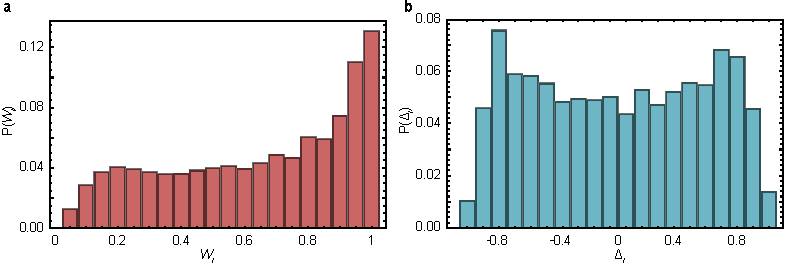
\includegraphics[width=\columnwidth]{figures/ch5/MBL_dists_combo.pdf} 
		\caption{\textbf{On-site potential histograms. a)} A histogram of the expected on-site potentials (red) from the applied quasi-periodic distribution. \textbf{b)} A histogram of the expected neighboring potential differences (blue) from the applied quasi-periodic distribution.}
		\label{fig:disHist}	
\end{figure}

\section{Breakdown of thermalization}

Our experimental protocol is very similar to that described in \S \ref{sec:ch4protocol} and is shown in Fig.~\ref{fig:ch5fig2}\textbf{b}. Our experiments begin in the Mott-insulating state with unity filling in a two-dimensional optical lattice. We first use the DMD to isolate a single, one-dimensional chain from the Mott insulator and then add the on-site potential offsets $h_i$. We then abruptly switch on the tunneling by reducing the lattice depth within a fraction of a tunneling time which realizes a quantum quench as in our previous study (Fig.~\ref{fig:ch5fig2}\textbf{c}). The final Hamiltonian parameters are given by a tunneling time $\tau=\hbar/J=4.3(1)\mathrm{ms}$ and $U = 2.87(3)J$ and remain constant for all experiments. We allow the system to evolve by unitary evolution in this Hamiltonian for a variable amount of time at the end of which we perform the same number-resolved imaging as in the previous chapter (\S \ref{sec:ch4protocol}). Since particle loss during the evolution of the system realizes a form of coupling to an external bath, we post-select on all images such that they contain the same number of atoms as intended for state initialization. In this way, we realize an on-site single-particle occupation fidelity of $99.1(2)\%$. This is limited by the fraction of doublon-hole pairs in the initial Mott insulator.\footnote{This number differs from the measured in-situ occupations of the unity-filling Mott-insulating shell. However, this is largely due to the loss during imaging that reduces this on-site fidelity and is not due to thermal excitations in the Mott insulator.} 

We first investigate the breakdown of thermalization in a subsystem that consists of a single lattice site. The conserved total atom number $N$ enforces a one-to-one correspondence between the particle number outcome on a single site $n_a$ and the outcome in the remainder of the system $n_b=N-n_a$ -- entangling the two subsystems via tunneling dynamics. Ignoring information about the remaining system makes the single-site a completely mixed state of different on-site occupation numbers. The associated number entropy is given by $S^{(1)}_n = -\sum_n p_n \log(p_n)$, where $p_n$ is the probability of finding $n$ atoms on the single-site. Due to the one-to-one correspondence mentioned above, this implies the lack of any off-diagonal (coherence) terms in the reduced density matrix. This is equivalent to saying that measuring the on-site number occupation for a single-site extracts all information available to that subsystem's reduced density matrix. Hence, $S^{(1)}_n$ is the single-site von Neumann entanglement entropy $S^{(1)}_{vN}$ as long as the system is globally pure.

\begin{figure}[t!]
		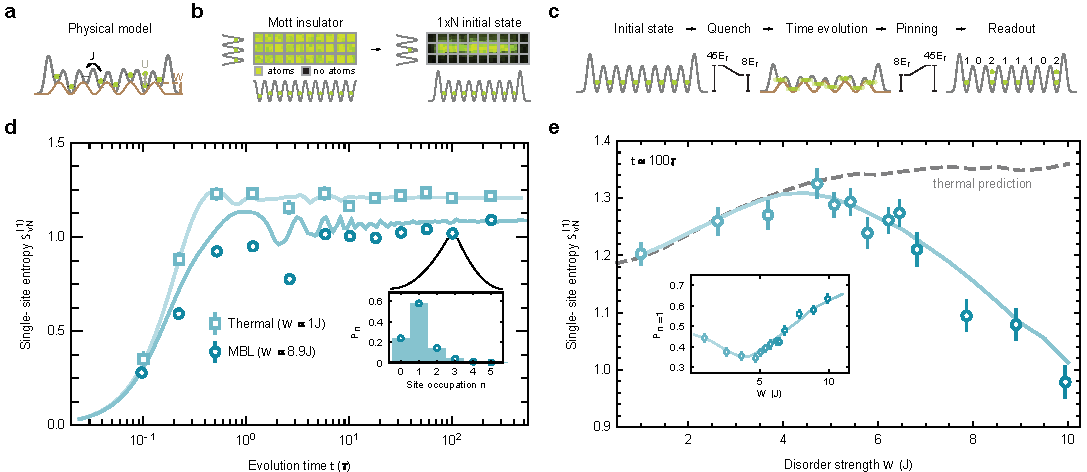
\includegraphics[width=\columnwidth]{figures/ch5/figure2.pdf} 
		\caption{\textbf{Breakdown of thermalization. a)} The physical model is illustrated here as an interacting Bose-Hubbard model with on-site potentials sampled from a quasi-periodic distribution. \textbf{b)} All experiments start from a unity-filling Mott-insulating state. The DMD is then used to create a single $1\times8$ site system. \textbf{c)} The quench protocol is outlined here where the $1\times8$ site initial state is evolved by unitary dynamics for a variable evolution time $t$ in the interacting Aubry-Andr\'e Hamiltonian. The state is then read out with single-site and number-resolved fluorescence imaging technique elucidated in \S \ref{sec:ch4}. \textbf{d)} The single-site von Neumann entropy, $S^{(1)}_{vN}(t)$, is plotted as a function of time for two different disorder strengths: $(W=1J)$, which corresponds to the thermalizing regime, and $(W=8.9J)$, which corresponds to the many-body localized regime. Note that the MBL regime has suppressed single-site entropy that persists up the longest evolution times. \textbf{e)} The measured single-site entropies at the end of the unitary evolution are then compared to the prediction by a thermal ensemble as a function of the applied disorder W. The single-site entropy agrees with the thermal prediction up to a finite disorder strength, at which point it becomes sub-thermal and consistent with numerics. The inset shows the probability of the site retaining exactly one atom, which is akin how well the site remembers the initial state. All solid lines are calculated by exact diagonalization. All error bars are the s.e.m.}
		\label{fig:ch5fig2}	
\end{figure}

Counting the atom number on an individual lattice site in different experimental realizations allows us to obtain the probabilities $p_n$ and compute $S^{(1)}_{vN}$. We performs such experiments for various evolution times. At a low disorder strength $(W=1.0(1)J)$, the entropy grows over a few tunneling times and then reaches a stationary value (Fig.~\ref{fig:ch5fig2}).\footnote{The naive assumption would be that the non-disordered regime should saturate in approximately a single tunneling time $\tau$. However, the plot in Fig.~\ref{fig:ch5fig2}\textbf{a} curiously saturates for this regime in $t\approx \frac{1}{2}\tau$. This is because of the fact that $J$ is defined for the field of the wave function and has the same consequence in the traditional Rabi problem where the oscillations happen with a frequency twice as fast as the driving field $\Omega$.} This stationary value is suppressed for larger disorder $(W=8.9(1)J)$ and remains constant over two orders of magnitude in evolution time. The lack of entropy increase indicates the absence of heating from an external source in the system -- as indicated by the agreement with the exact diagonalization calculations of the coherent dynamics up to longest measured evolution times.

To determine the effect of disorder strength on this saturated value, we measure the $S^{(1)}_{vN}(W,t=100\tau)$ in Fig.~\ref{fig:ch5fig2}\textbf{e}. To evaluate the degree to which this agrees with local thermalization, we compare the result with the prediction of a microcanonical thermal ensemble for our system (compare predictions from previous chapter \S \ref{sec:ensPredict}). For weak disorder, the measured entropy agrees with the prediction of a thermodynamic ensemble up to a finite disorder strength -- we use this agreement to identify this regime a ``thermalizing" one. As disorder is increased, we observe an increasingly large departure from the the prediction of thermal equilibrium. This sub-thermal regime retains memory of the initial state which initially has no on-site fluctuations and therefore reduced entropy in comparison to the thermal prediction. The degree to which the single-site relaxation differs from this thermal prediction increases for stronger disorder. This memory of the initial state (Fig.~\ref{fig:ch5fig2}\textbf{e} inset) is the same metric by which other experiments of localization in interacting systems have measured a lack of thermalization \cite{Schreiber2015,Bordia2016,Smith2016,Choi2016,Luschen2017}.

\section{Localization of particles}

This observed breakdown of thermalization is expected to be a consequence of the spatial localization of the constituent particles in the system. For point-like interactions between particles, particle transport becomes a necessary condition for exchange of energy to allow relaxation towards equilibrium. The lack of such transport has been previous observed as a localization length of an initially prepared density step into empty space \cite{Choi2016}. We simultaneously measure this localization as well as the breakdown of thermalization by directly probing density-density correlations within the system while maintaining the average density in the system. These correlations are captured by $G^{(2)}(d) = \langle n_i n_{i+d} \rangle - \langle n_i \rangle \langle n_{i+d} \rangle$, where $\langle ... \rangle$ denotes simultaneously averaging over different disorder realizations as well as all sites $i$ of the chain. The particle number on two sites at distance $d>0$ are uncorrelated for $G^{(2)}(d) = 0$. If a particle is coupled to a site a distance $d$ away, then the sites become anti-correlated, and the correlator decreases to $G^{(2)}(d)<0$.

An important contribution to these correlations relates to the structure of the applied on-site potentials themselves. The on-site potential $h_i$ has a non-vanishing autocorrelation function $A(d)=\langle h_i h_{i+d} \rangle_i $ (Fig.~\ref{fig:g2Fit}\textbf{b}) at all distances that is inherited by the fluctuations in the density-density correlations that we need to account for when extracting the localization length $\xi$. From this we construct an ansatz fit function:

\begin{equation}
\label{eqn:g2fit}
G^2(d)= (a + b\times A(d))e^{-d/\xi}
\end{equation}

 which is shown on top of the data and exact theory in Fig.~\ref{fig:g2Fit}\textbf{c}. We exemplify how we extract a length scale from the measured the density-density correlations $G^{(2)}(d)$ in Fig.~\ref{fig:g2Fit}: we show a comparison of the measured correlations, the exact diagonalization, and the ansatz for the functional form (\ref{eqn:g2fit}) of the correlations.

\begin{figure}[t!]
		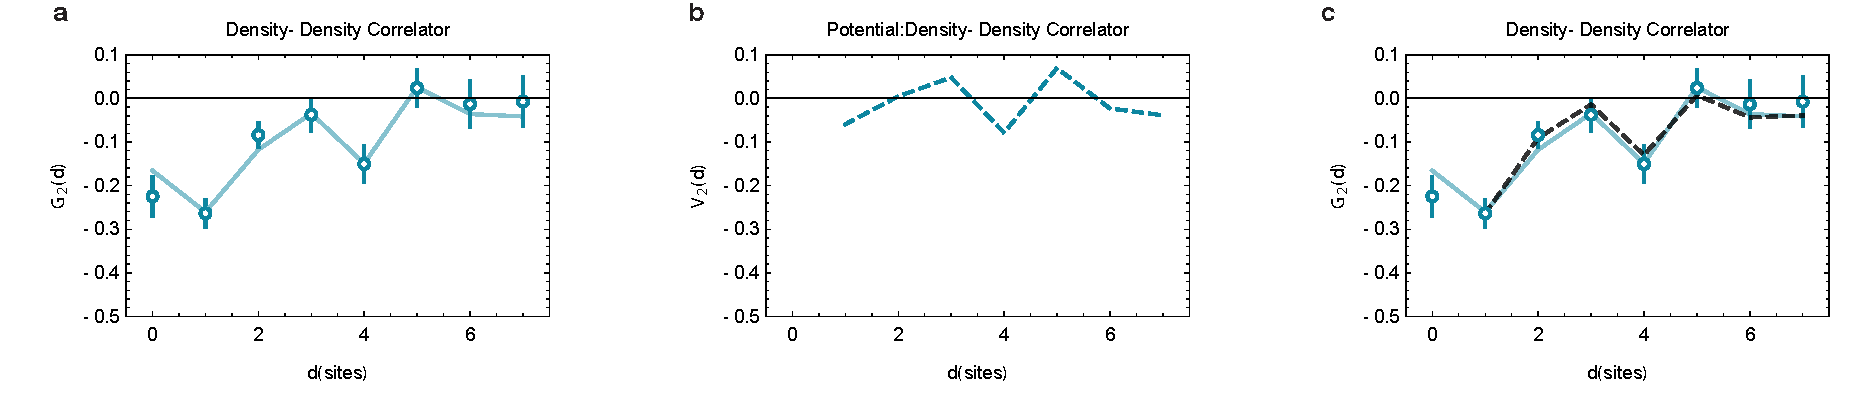
\includegraphics[width=\columnwidth]{figures/ch5/G2Combo_Row_2edit.pdf} 
		\caption{\textbf{$G_2$ data, theory, and fit function. a)} The raw data and exact theory are plotted after an evolution time $t=100\tau$ at a disorder strength $W=4.8(1)J$. \textbf{b)} The autocorrelation function of the on-site potential distribution, $A(d)=\langle h_i h_{i+d} \rangle_i $, is plotted as a function of inter-site distance. \textbf{c)} Combines the measured data, the exact theory, and the ansatz fit function (\ref{eqn:g2fit}) that incorporates the autocorrelation function of the on-site potentials. The theory is calculated by exact diagonalization. The error bars are the s.e.m.}
		\label{fig:g2Fit}	
\end{figure}

From these fits we extract the correlation length $\xi$ from the long-time saturated correlations to probe the relationship between disorder strength and localization. At low disorder ($W=1J$), we find these correlations to be independent of distance and at a constant, negative offset. This indicates that the particles are able to tunnel across the entire system and hence are delocalized (Fig.~\ref{fig:ch5fig3}\textbf{c}). In the regime of strong disorder ($W=7.9J$), only nearby sites show significant correlations and demonstrate the suppression of particle motion across large distances. We thus conclude that the particles are localized in this regime. We then plot the extracted localization length $\xi$ as a function of disorder in Fig.~\ref{fig:ch5fig3}\textbf{c} where the correlation length exists at the system size limit until a finite disorder strength where it is reduced to the smallest measured value of $\approx 1$ site.

\begin{figure}[t!]
		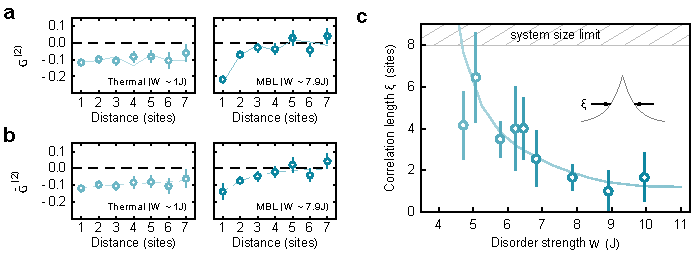
\includegraphics[width=\columnwidth]{figures/ch5/figure3_editv2edit.pdf} 
		\caption{\textbf{Localization. a)} The measured two-point correlations, $G^{(2)}(d)$, are plotted for both the thermalizing $(W=1J)$ and MBL $(W=7.9J)$ regimes. \textbf{b)} By removing the non-monotonic behavior of the on-site potential correlations we visualize the localization of the distribution $\tilde{G}^{(2)}(d) = G^{(2)}(d) - b\times A(d) e^{-d/\xi}$. \textbf{c)} The extracted correlation length $\xi$ is then plotted as a function of disorder depth W. This correlation length $\xi$ becomes smaller than the system size at the same finite disorder at which thermalization breaks down in the system. All solid lines are calculated from exact diagonalization. The dashed lines are the results of a a fit (\ref{eqn:g2fit}). The error bars are the s.e.m.}
		\label{fig:ch5fig3}	
\end{figure}

The observation of localized particles is a consistent with the description of MBL in terms of local integrals of motion \cite{Serbyn2013a,Serbyn2013b,Huse2014}. This model was initially formulated for MBL in a spin system, but can be extended to lattice bosons. It describes the global eigenstates as a product of exponentially localized orbitals. The correlation length extracted from our model is a measure of these orbitals. Since the latter form a complete set of locally conserved quantities that prohibit an ergodic exploration of all available phase space with respect to global thermodynamic constraints(total energy, total particle number, etc.), this picture connects the breakdown of thermalization in MBL with integrable systems.

\section{Entanglement dynamics in an interacting, many-body localized system}

Up till this point, the role of interactions in this many-body system has been solely related to the concept of thermalization and non-integrable systems. However, since non-interacting systems are already known to Anderson localize it may seem like purely a competition of two effects in this system: i) thermalization when disorder is low and interactions and transport realize ergodic, thermal eigenstates, and ii) localization when disorder is so large that it is the dominates energy scale and effective breaks up the system into a series of disconnected, localized, non-interacting chunks. However, this picture was shown by Bardarson \emph{et al.}\cite{Bardarson2012} as an inaccurate description of the system. In this pioneering theory work, it was shown how the bipartite entanglement entropy dynamics of a disordered spin system differs between a non-interacting and an interacting system. A non-interacting system only realizes the rapid relaxation akin to the observed single-site entropy measured in Fig.~\ref{fig:ch5fig2}. However, any infinitesimal interaction between particles/spins will lead to long term entanglement growth that is logarithmically slow with time. This result led to the identification of the logarithmically slow entanglement growth as the distinguishing behavior that realizes the unique characteristics of a strictly interacting\footnote{Nearly all literature or researchers in this field will exclude this ``interacting" descriptor. Strictly speaking, a system of many, non-interacting bodies would also localize (i.e. Anderson localization) and is the exact comparison given in Bardarson, \emph{et al.}. However, it is the fact that the many-bodies interact at all that give rise to the unique dynamics and so I add this qualifier here for emphasis and clarity only.}, many-body localized system.\footnote{An additional comment is that a significant distinction here is that \emph{both} regimes, delocalized and the localized, can be provably shown to be interacting ones. Non-interacting systems without disorder will be delocalized but are also strictly non-thermalizing systems: the energy per particle is an additional, extensive constraint on the system and once again realizes an integrable system. Therefore, simply demonstrating that a system delocalizes or localizes are \emph{in}sufficient observables -- although they are considered to be necessary ingredients for thermalization and its breakdown, respectively. In a many-body localized system, it is the logarithmically slow entanglement growth that defines the system as being localized in the presence of interactions.}

Discerning the unique entanglement growth in a many-body localized system requires a precise understanding of how correlations can develop due to unitary evolution of this pure quantum state. In a Bose-Hubbard chain with fixed global particle number, there are two classes of degrees of freedom that contribute to the bipartite entanglement entropy: i) the number of particles in a given subsystem, and ii) the way those particles are configured among the available lattice sites in the subsystem. Mathematically, this can be separated exactly for the von Neumann entropy, $S_{vN} = S_n + S_c$. This becomes clear if we consider the reduced density matrix $\rho_A$ of subsystem A in the Schmidt basis $\rho_{ii}$:

\begin{equation}
\label{eqn:svn_rhoii}
S_{vN} = \sum_i \rho_{ii} \log \left( \rho_{ii} \right)
\end{equation}

Since the global particle number is conserved, the same argument for a single-site having no coherences between different particle numbers in a subsystem holds also for larger subsystems; there is again a one-to-one, unique relationship between with a given number of particles in subsystem A and subsystem B ($N_A, N_B=N-N_A$). This permits us to break up (\ref{eqn:svn_rhoii}) into a double sum over the particle number $n$ in a given subsystem and then all states $i$ within that manifold:

\begin{equation}
\label{eqn:svn_blk}
S_{vN} = \sum_{n=0}^N \sum_i p_n \rho^{(n)}_{ii} \log \left ( p_n \rho^{(n)}_{ii} \right )
\end{equation}

where $p_n$ refers to the probability of a populating the manifold of $n$ atom states in subsystem A. This can be understood graphically (see Fig.~\ref{fig:sepSvn}a) as the reduced density matrix being a block diagonal matrix where the population of each block is given by $p_n$ and each respective block within the $n$ atom manifold $\left ( \rho^{(n)}_{ii} \right )$ may be individually diagonalized and normalized $\left ( \sum_i \rho^{(n)}_{ii} = 1\right )$.\footnote{In the single-site regime, each of these blocks $\rho^{(n)}_{ii}$ is reduced to containing only a single state. Since this block has only one entry it cannot have any internal coherences. Hence, measuring single-site occupation number is all the information available.} By exploiting the lack of coherences between blocks and the normalization of each block, $S_{vN}$ can be reduced to a sum of two separate contributions: $S_n$ and $S_c$ (\ref{eqn:svn_sep}).

\begin{equation}
\begin{aligned}
S_{vN}&=\sum_{n=0}^N \sum_i p_n \rho_{ii}^{(n)} \left[\log{\left ( p_n \right )} + \log {\left ( \rho_{ii}^{(n)} \right )} \right] \\
&=\sum_{n=0}^N p_n \log{\left ( p_n \right )} \sum_i \rho_{ii}^{(n)} + \sum_{n=0}^N p_n \sum_{i} \rho_{ii}^{(n)} \log {\left ( \rho_{ii}^{(n)} \right )} \\
&=\sum_{n=0}^N p_n \log{\left ( p_n \right )} + \sum_{n=0}^N p_n \sum_{i} \rho_{ii}^{(n)} \log {\left ( \rho_{ii}^{(n)} \right )} \\
&=S_{n} + S_{c}.
\end{aligned}
\label{eqn:svn_sep}
\end{equation}

This separation of contributions to entanglement by types of correlation between the two subsystems gives rise to exactly the separation of identifying behavior in many-body localization (Fig.\ref{fig:sepSvn}). It also qualitatively reflects the original results presented in \emph{Bardarson, et al.}\cite{Bardarson2012} and distinguishes between the contributions to entanglement from atom delocalization, which can arise in a non-interacting system ($S_n$), and the contribution from atom-atom interactions that gives rise to a persistent growth of entanglement ($S_c$).

\begin{figure}[t!]
		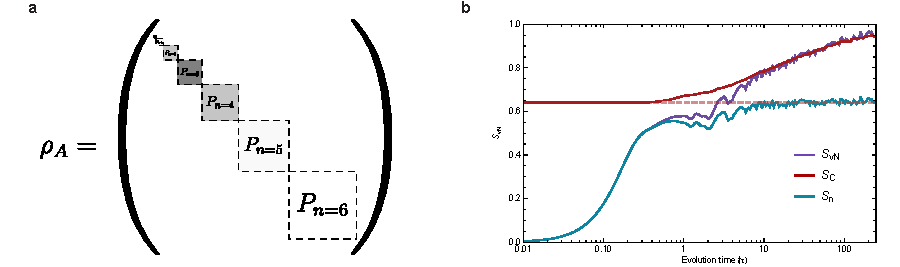
\includegraphics[width=\columnwidth]{figures/ch5/combo_sep_svn.pdf} 
		\caption{\textbf{Degrees of freedom and entropy. a)} Shows an illustration for the reduced density matrix $\rho_A$ of a system where the subsystem size is larger than a single lattice site. The size of the blocks in this system refer to the Hilbert space within the manifold of states that contain $n$ atoms in the subsystem. The shading refers to the probability of populating states in that block, $P_n$. \textbf{b)} The bipartite von Neumann entropy plotted is for half-size subsystem with a total size of $L=6$ sites. The separate contributions to this entropy, $S_n$ and $S_c$, provide independent metrics for distinguishing the rapid relaxation and the slow, non-local correlations built up by the presence of interactions in the system. The solid lines are produced for exact diagonalization.}
		\label{fig:sepSvn}	
\end{figure}

The entropy generated by fluctuations in particle number in a given subsystem is suppressed by the presence of localization and has the same early-time saturation behavior as for single-site in the system. The entropy associated with configurations of particles within a given block of the density matrix, however, can still slowly develop correlations with the remainder of the system and is solely responsible for the logarithmically slow entropy growth used to distinguish interacting, many-body-localized systems.

This separation of correlation contributions additionally provides some intuition for discerning the difference in the dynamics of Anderson localized, many-body localized, and thermalizing systems. In a thermalizing system, the lack of disorder allows for particle to rapidly transport through the whole system, and build correlations between the two subsystems by both particle exchange across the subsystem boundary, and interactions between particles that cause correlations between particular configurations in the two subsystems. 

\subsection{Phenomenological description of localized orbitals: non-interacting} 

To better elucidate how entanglement develops in these localized systems, we will refer to a phenomenological model adapted from spin systems to a Bose-Hubbard, which is written in the physical on-site basis below:

\begin{equation}
\label{eqn:andyham}
\hat{H} = -J\sum_i \left ( \hat{a}_i^\dagger \hat{a}_{i+1} + h.c. \right ) + W \sum_i h_i \hat{n}_i
\end{equation}

In this Anderson localized (i.e. non-interacting) regime, the particles are exponentially localized to their initial site by disorder. We will assume we are in the regime $W\gg J$ for simplicity. This localization hints to the fact that eigenstates of the system may be built out of a product of creation operators that populate such localized orbitals with individual atoms $\hat{\mathcal{A}}_k^\dagger$.\footnote{This concept is intentionally presented to be similar to populating local local Wannier functions in a lattice with $\hat{a}^\dagger$, which it will reduce to in the infinitely-deep disorder limit as $\xi\rightarrow 0$.} We can find much of the phenomenological physics by expressing such an exponential orbital a superposition of on-site creation operators with exponentially decreasing amplitude. We can think of eigenstates of this system as being built out of quasi-local creation operators: 

\begin{equation}
\hat{\mathcal{A}}_k^\dagger \sim \frac{1}{\mathcal{N}} \sum_j \hat{a}_j^\dagger e^{i \phi_j} e^{-| x_j - x_k |/\xi }
\label{eqn:AHAT}
\end{equation}

where the only degree of freedom being the phase $\phi_j$ of the exponentially decaying amplitude on these sites and enables these orbitals to be constructed such that they are orthogonal $\left ( \langle 0 | \hat{\mathcal{A}}_{j\neq k} \hat{\mathcal{A}}^\dagger_k |0\rangle = 0 \right )$. In the Anderson localized case, the exponentially localized particles are eigenstates of the non-interacting disordered Hamiltonian and only these many-body phases evolve in time. This evolution happens because of the local potential offsets $\tilde{W}_k$ they experience and therefore can be described by an effective Hamiltonian:

\begin{equation}
\hat{H}^{eff} \sim \sum_k \tilde{W}_k \hat{\mathcal{A}}_k^\dagger \hat{\mathcal{A}}_k
\label{eqn:ahatHam}
\end{equation}

Note that this effective Hamiltonian is diagonal in the basis of the occupation number of localized orbitals $\hat{\mathcal{A}}_k^\dagger \hat{\mathcal{A}}_k$ and therefore, in this localized orbital basis, creating such an eigenstate will evolve in a global phase. Let us consider a simple initial state that is separable but in a superposition of these localized orbitals:
 
 \begin{equation}
 |\psi_o\rangle =\frac{1}{\mathcal{N}} \left (I+\hat{\mathcal{A}}_0^\dagger \right )|0_0\rangle \otimes \left ( I+\hat{\mathcal{A}}_1^\dagger \right ) |0_1 \rangle 
 \end{equation}
 
 In the case of a non-interacting system, the temporal dynamics of this initial state simply depend upon the local orbital occupation number:
 
 \begin{equation}
 |\psi_o (t) \rangle =\frac{1}{\mathcal{N}} \left (|0_0\rangle + e^{i \tilde{W}_0 t} |1_0 \rangle \right ) \otimes \left (|0_1\rangle + e^{i \tilde{W}_1 t} |1_1 \rangle \right ) 
 \label{eqn:psi_time}
 \end{equation}
 
In the basis of the localized orbitals, the dynamics of the system are entirely contained in the local phase evolution of the populated orbital and preserve the separability of the initial state -- they remain unentangled at all times. Importantly, however, in the basis of physical lattice sites, such a state would still retain some entanglement from particle number fluctuations across a real-space bipartition that cuts through all the $\mathcal{A}^\dagger_k |0\rangle$ states at some physical site index. In fact, our original formulation of $\hat{\mathcal{A}}_k^\dagger$ (\ref{eqn:AHAT}) as an exponentially decaying amplitude of on-site creation operators $\hat{a}_k^\dagger$ suggests (correctly it turns out) that eigenstates have an area-law scaling of entanglement entropy (\S \ref{sec:ch3}). Importantly, though this entanglement does not grow as a function of time (\ref{eqn:psi_time}).
 %However, when evaluated in the bare basis of on-site occupations $\hat{a}^\dagger_j$ the phases $\phi_j$ will continue to evolve.

% \[
% |\psi_o\rangle =\frac{1}{\mathcal{N}} \left (I+\hat{\mathcal{L}}_0^\dagger \right ) \otimes \left ( I+\hat{\mathcal{L}}_1^\dagger \right ) |0_0 0_1 \rangle = \frac{1}{\mathcal{N}} \left ( |0_0 0_1 \rangle +  |0_0 1_1 \rangle + |1_0 0_1 \rangle + |1_0 1_1 \rangle \right )
% \]

\subsection{Phenomenological description of localized orbitals: \emph{interacting}} 

We will use conceptually expand the framework presented above to think about the interacting regime by adding very weak but non-zero interactions:

\begin{equation}
\label{eqn:mblham}
\hat{H} = -J\sum_i \left ( \hat{a}_i^\dagger \hat{a}_{i+1} + h.c. \right ) + \frac{U}{2} \sum_i \hat{n}_i \left (\hat{n}_i - 1 \right ) + W \sum_i h_i \hat{n}_i
\end{equation}

In this many-body localizing Hamiltonian, we will work in the regime where $W\gg J \gg U$. We see from the formulation above that the interaction occurs for multiply occupied sites in the physical basis. Attempting to adapt our intuition of the eigenstates from the non-interacting basis, we would suspect that in this weakly interacting limit the system will still be constructed out of localized orbitals. The difference being that where orbitals overlap they will see an energy shift due to the particle-particle interaction that exists in our bare physical basis:

\begin{equation}
U^{eff}_{j,k} \sim \frac{U}{2} \sum_i e^{-| x_i - x_k |/\xi } e^{-| x_i - x_j |/\xi } \sim \tilde{U} e^{-| x_j - x_k |/ \xi}
\label{eqn:ueff}
\end{equation}

where we only include overlap from two orbitals centered about sites-$j$ and $k$ since overlap with successively more orbitals will exponentially decrease in strength.\footnote{They may need to be considered in terms of finding the correct quantitative values for the dynamics of a system, but to see the phenomenological dynamics we can stop at this second-order non-local interaction.} It remarkably turns out that this concept is approximately true and we can again reconstruct eigenstates form localized quantities\cite{Serbyn2013a,Serbyn2013b,Huse2014}\footnote{It is very tempting to assume $\hat{\mathcal{L}}^\dagger_k \sim \hat{\mathcal{A}}^\dagger_k$. However, this is importantly not the case. It is the many-body states that are hybridized by the interactions $ \left (\text{i.e.~} \hat{\mathcal{L}}^\dagger_j \hat{\mathcal{L}}^\dagger_k |0\rangle \sim \left ( \hat{\mathcal{A}}^\dagger_j \hat{\mathcal{A}}^\dagger_k  + \alpha \hat{\mathcal{A}}^\dagger_j \hat{\mathcal{A}}^\dagger_j + \alpha' \hat{\mathcal{A}}^\dagger_k \hat{\mathcal{A}}^\dagger_k + ...   \right ) |0\rangle \right )$. The new localized quantities will share atoms from these original non-interacting orbitals and make it difficult to directly compose in these non-interacting terms. Although, they will appear relatively close if only looking at on-site occupation number. This example is further explained in Appendix : \ref{appendix:Ch6Cal}.} which we will now construct from new creation operators $\hat{\mathcal{L}}^\dagger_k$.  We can incorporate this interactions into our new Hamiltonian built out of our new localized creation operators below:

\begin{equation}
\hat{H}^{eff} \sim \sum_k \tilde{W}_k \hat{\mathcal{L}}_k^\dagger \hat{\mathcal{L}}_k + \sum_{j,k} U^{eff}_{j,k} \hat{\mathcal{L}}_j^\dagger \hat{\mathcal{L}}_j\hat{\mathcal{L}}_k^\dagger \hat{\mathcal{L}}_k
\label{eqn:hamMBL}
\end{equation}

While this Hamiltonian also has eigenstates that are constructed out of quasi-local creation operators ($\mathcal{L}^\dagger_k$), the evolution of the phases now depends upon a non-local interaction term between the population of spatially separated, localized orbitals. In particular, if we return to our original initial state example, $|\psi_o\rangle$, the dynamics of the many-body states will no longer remain separable:

 \begin{equation}
 |\psi_o (t) \rangle = \frac{1}{\mathcal{N}} \left ( |0_0 0_1 \rangle +  e^{i \tilde{W}_1 t} |0_0 1_1 \rangle + e^{i \tilde{W}_0 t} |1_0 0_1 \rangle + e^{i \left ( \tilde{W}_0 + \tilde{W}_1 \right ) t} e^{i U_{0,1}^{eff} t}|1_0 1_1 \rangle \right )
 \label{eqn:mbl_time}
 \end{equation}

Their is now an additional phase evolution from $e^{i U_{0,1}^{eff} t}$ that will make the system inseparable in this localized orbital basis and the physical site basis -- exemplifying the entangling of the states due to the interaction term. This interaction is physically derived from the the additional energy offset that atoms experience from multiply occupied sites that, in this case, will depend on the relative overlap of exponentially localized particles. This simple, phenomenological model not only describes how the system becomes entangled but qualitatively characterizes from the phase $e^{i U_{x_j,x_k}^{eff} t}$ that this entanglement will happen logarithmically slowly throughout the system since the interaction is exponentially weak between distance sites $d$ apart:

\begin{equation}
\tau_{ent} U_{x_j,x_{j+d}}^{eff} = \tau_{ent} \tilde{U} e^{- d/ \xi} \sim 1 \rightarrow \log{ \left [ \tau_{ent} \tilde{U} \right ] } \xi \sim d 
\label{eqn:utime}
\end{equation}

This framework is adapted from the ``l-bit" description used to provide a phenomenological picture for the entanglement dynamics of many-body localization in a spin system \cite{Serbyn2013a,Serbyn2013b,Huse2014}.\footnote{Strictly speaking, the ``l-bit" (localized bit) picture from spins is somewhat inadequate since the on-site degree of freedom in the Bose-Hubbard case can take on more than two values. This is why an attempt at a modification to this picture has been added above for the population of these localized orbitals with a creation operator $\mathcal{L}^\dagger_k$ where multiple on-site occupations can apply. The additional translation of this model is that the ``p-bits" (physical bits) are now defined as the bare on-site occupation basis given by creation operators $\hat{a}^\dagger_k$. Lastly, the original ``l-bit" picture, as written for spins, is that quasi-local operators are defined as to be comprised of eigenstates that commute with a product of local Pauli operators (e.g. $... I_{k-2} \sigma_{k-1}^{(z)} \sigma_{k}^{(x)} \sigma_{k+1}^{(y)} I_{k+2} ...$) in the ``p-bit" basis. However, it should be repeated once more that this is purely a phenomenological picture to help with intuitively writing down a mathematical description of the observed behavior in the system, not a literal diagonalization.} The implication of the framework presented above is that the magnitude of local fluctuations in particle number are entirely restricted by the localization length scale $\xi$. The scaling behavior of entanglement within a single eigenstate of this many-body localized is again an area law -- like the Anderson localized case discussed above. However, if the initial state is a superposition of several of these local creation operators $(\hat{\mathcal{L}}^\dagger_k)$ the system will eventually become entangled by this interaction term and converge to a volume law.

Importantly, our initial state is not an eigenstate of the final Hamiltonian in this localized basis and hence the relative phase evolution of eigenstates that are sensitive to the exact population of these localized orbitals that results in the slow entanglement among the localized constituents of the system. From this framework we can additionally find an intuitive description of the spread of entanglement after a quench throughout the system for the thermalizing, Anderson localized, and many-body-localized systems (Fig.~\ref{fig:ch5fig1}). In the thermal case, the system rapidly develops entanglement of both types that extend across the entire system. The Anderson-localizing system develops entanglement only due to the finite extent of particle delocalization across a boundary and therefore all entanglement is additionally local in the system. The many-body-localized system develops initial entanglement due to the particle number fluctuations, similar to that of the Anderson-localized system, but also develops entanglement among the local configurations of particles in the system that slowly spreads across all length scales. This entanglement of local configurations of particles is in part possible because it respects the locally conserved integrals of motion. However, it can still scramble initial phase relationship of these quasi-local operators throughout the entire system, albeit logarithmically slowly due to the exponentially small overlap between distant orbitals.

\begin{figure}
\floatbox[{\capbeside\thisfloatsetup{capbesideposition={left,top},capbesidewidth=2 in}}]{figure}[\FBwidth]
{\caption{\textbf{Separation of entanglement in Bose-Hubbard. a)} These illustrations depict the separate contributions to the entanglement (\ref{eqn:svn_sep}) in a Bose-Hubbard system. \textbf{b)} The role of these contributions qualitatively differ for these regimes: i) in a thermalizing system, both the number and configurational entanglement grow rapidly together and throughout the entire system, ii) the Anderson localized regime possesses only number entanglement which remains local, iii) the many-body-localized regime possesses local number entanglement but also harbors a logarithmically slow growth of configurational entanglement throughout the system.}\label{fig:ch5fig1}}
{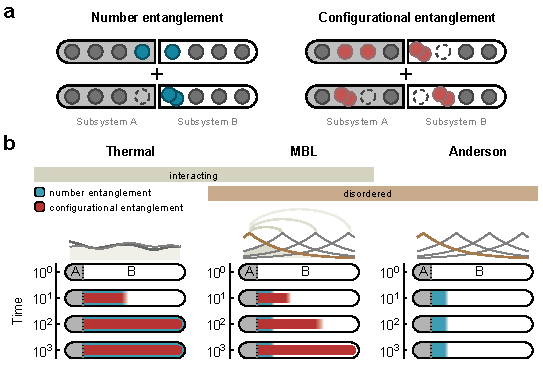
\includegraphics[width=4 in]{figures/ch5/figure1.pdf}} 
\end{figure}

%\textcolor{red}{consider working out example for conserved localized orbital number}

\subsection{Measured entanglement dynamics}

While we have access to the atom number in a given subsystem, $p_n$, which allows us to directly compute $S_n$ for any given subsystem, we do not have access to the entropy of configurations $S_c$. Therefore, we probe this entanglement from the underlying correlations of configurations between the bipartite subsystems. This correlation of configurations must be performed respective to the local manifold of conserved atom number in a given system. We define this configurational correlator as a measure of non-separability between configurations $A_n$ and its compliment $B_{n'}$ with $n$ particles in A and $n'=N-n$ particles in B:

\begin{equation}
\label{eqn:cab}
C=\sum_{n=0}^N p_n \sum_{\{A_n\},\{B_{n'}\}} \left | p \left ( A_n B_{n'} \right ) - p \left ( A_n \right ) p \left (B_{n'} \right ) \right |
\end{equation}

where $p \left ( A_n B_{n'} \right ) $ is the joint probability of a particular Fock state configuration $A_n B_{n'}$ occurring and $p \left ( A_n \right )$,$p \left (B_{n'} \right )$ are the marginal probabilities of the local Fock state configurations $A_n$, $B_{n'}$ occurring independently. A non-zero $C$ provides a strict statement that the two subsystems are not separable within their configurational degrees of freedom and therefore implies entanglement of the configurational type. What this non-zero value implies mathematically is an upper bound on the magnitude of the coherence terms within the blocks of the reduced density matrix in Fig.~\ref{fig:sepSvn}. Importantly, this configurational correlation $C$ is numerically found to be almost linearly proportional with $S_c$ for our parameter regimes (Fig.~\ref{fig:CABsc}). However, this proportionality is not always linear and some discussion about the mathematical bounds involving this correlator ($C$) are discussed in Appendix \ref{appendix:Ch5Cal}.

\begin{figure}[t!]
		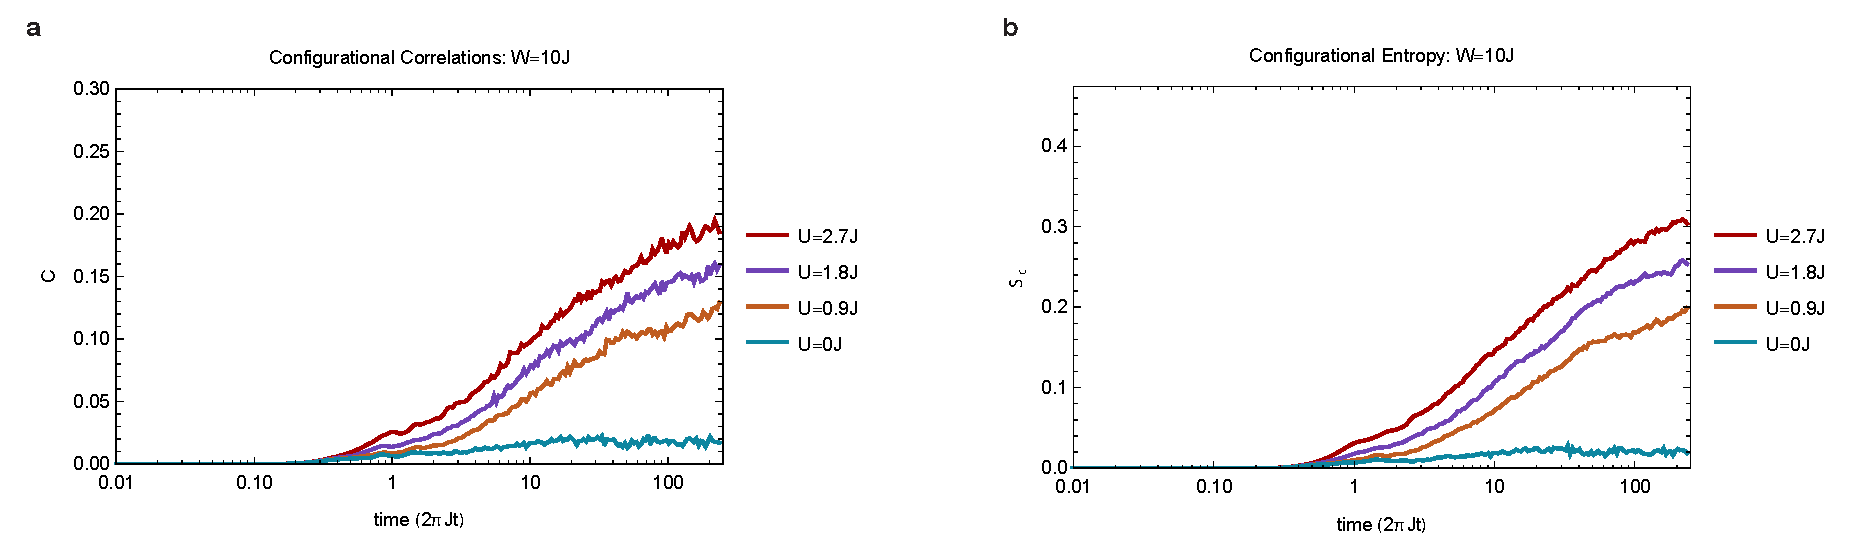
\includegraphics[width=\columnwidth]{figures/ch5/CAB_SC_Row_ins_2.pdf} 
		\caption{\textbf{$C$ and $S_c$. a)} The calculated configurational correlations are plotted for various interaction strengths in the MBL regime ($W=10J$). \textbf{b)} The calculated configurational entropy are plotted for various interaction strengths in the MBL regime ($W=10J$). Both calculations are for a $6$-site system where we find excellent qualitative agreement between the two metrics. Note that a small amount of configurational correlation exists in the non-interacting case, but never grows. The finite value here is due to the many-body nature of the non-interacting system which still harbors bosonic statistics that effect this configurational correlation. However, since it requires overlap of the particles, it is highly suppressed with localization length $\xi$. In the interacting case this changes the final saturation value but not the growth. All calculations are performed by exact diagonalization.}
		\label{fig:CABsc}	
\end{figure}

Due to the ability to resolve the exact Fock state distribution with our microscope, we study the time dynamics for both the particle number entropy ($S_n$) and the configurational correlations ($C$). We study all temporal dynamics within a $6$-site Bose-Hubbard system. Without disorder, we find that both $S_n$ and $C$ indeed grow rapidly and reach a stationary value within a few tunneling times (Fig.~\ref{fig:ch5fig4}\textbf{a}). In the presence of strong disorder, we find a qualitatively different behavior for both quantities. Again, $S_n$ reaches a stationary state, although after longer evolution time due to reduced effective tunneling. Additionally, the stationary value is significantly reduced (approximately a factor of 2 in Fig.~\ref{fig:ch5fig4}\textbf{a,b}) and indicates the the suppression of particle transport in the system. The correlator $C$, in contrast, shows a persistent slow growth up to the longest evolution times reach by our measurements (Fig.~\ref{fig:ch5fig4}\textbf{b}). The growth is consistent with logarithmic behavior over two decades of evolution time. We conclude that we observe the interaction-induced entanglement dynamics in the MBL regime, which is additionally consistent with the phenomenological model presented earlier\cite{Bardarson2012,Serbyn2013a,Serbyn2013b,Huse2014}. The agreement of the longterm dynamics of $S_p$ and $C$ with numerical calculations in the MBL regime confirms the unitary evolution of the system and is consistent with very few scattering events that could decohere the system ($\gamma \leq 1$ photon / (second $\cdot$ atom number),  \S \ref{sec:ch5dec}).

\begin{figure}[t!]
		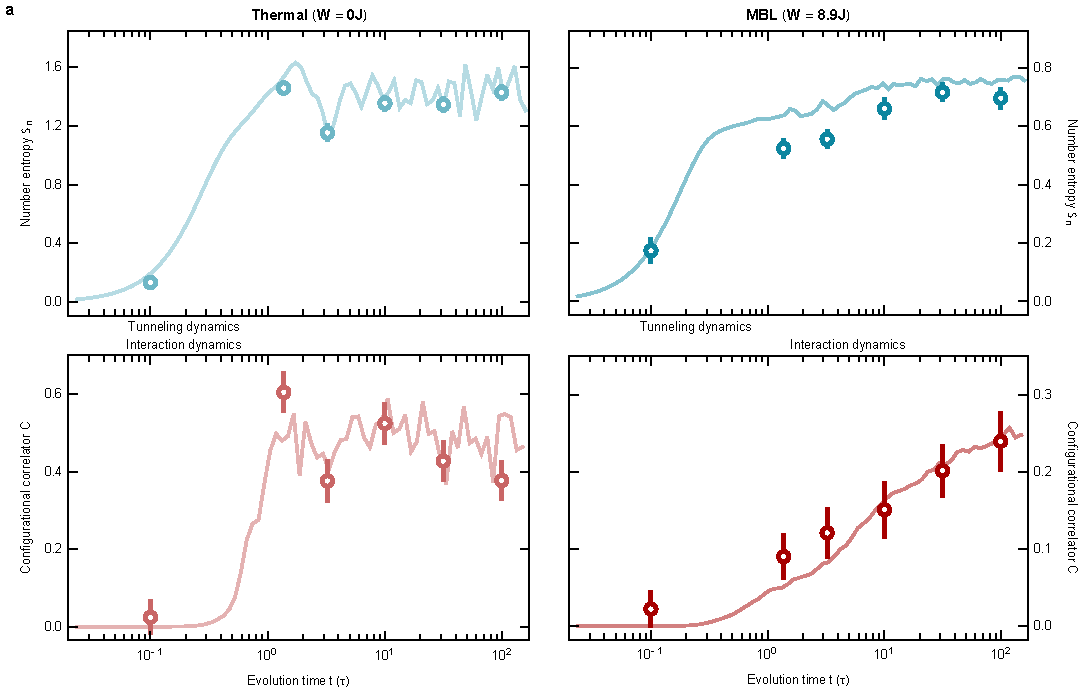
\includegraphics[width=\columnwidth]{figures/ch5/figure4_raw.pdf} 
		\caption{\textbf{Separation of entanglement. a)} Both the measured number entanglement entropy (blue) and the configurational correlator (red) are plotted for a $6$-site Bose-Hubbard system after a quench with no disorder -- realizing a thermalizing system. Note that both contributions to the entanglement in the system rapidly grow and saturate within a single tunneling time $\tau$. The configurational correlations, requiring some amount of local number fluctuations, turning on more rapidly, but after the start of the number entropy growth. \textbf{b)} Both the measured number entanglement entropy (blue) and the configurational correlator (red) are plotted for a $6$-site Bose-Hubbard system after a quench with strong disorder ($W=8.9J$) -- realizing a many-body-localized system. The number entanglement entropy rapidly grows and saturates within $10\tau$ while the configurational correlations give rise to a logarithmically slow growth consistent with the phenomenological model expectations of MBL. All solid lines are calculated by exact diagonalization. All error bars are the s.e.m.}
		\label{fig:ch5fig4}	
\end{figure}

Considering the scaling of this entropy in subsystems of different sizes provides us additional insights into the spatial distribution of entanglement in the system: in a one-dimensional system, locally generated entanglement results in a subsystem size independent entropy, whereas entanglement from non-local correlations causes the entropy to increase in proportion to the size of the subsystem. In reference to the subsystem's boundary and volume, these scalings are called area law and volume law. We find almost no change in $S_n$ for different subsystems of an $8$-site MBL system (Fig.~\ref{fig:ch5fig5}\textbf{a}) -- indicating an area law scaling to the localization of the particles and confirming the suppression of particle transport. In contrast, the configurational correlations $C$ increase until the subsystem reaches half the system size (Fig.~\ref{fig:ch5fig5}\textbf{b}). Such a volume-law scaling is also expected for the entanglement entropy and demonstrates that the observed logarithmic growth indeed stems form non-local correlations across the entire system. \footnote{This volume-law scaling of the configurational correlations, and therefore the von Neumann entropy, is a result of the unitary dynamics in the system. In fact, each individual eigenstate in the MBL system actually only harbors area-law entanglement. It is the unitary evolution of a superposition of many MBL eigenstates that give rise to this volume-law scaling.}

\begin{figure}[t!]
		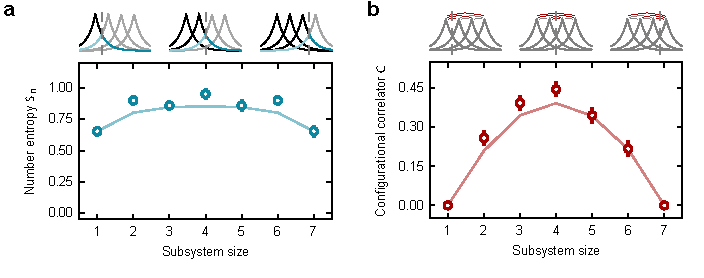
\includegraphics[width=\columnwidth]{figures/ch5/figure5_edit.pdf} 
		\caption{\textbf{Subsystem-size scaling of entanglement entropy. a)} The particle number entropy, which is most sensitive to the distance over which particle number fluctuations are possible, proves very insensitive to subsystem-size scaling and indicates the existence of an area law caused by particle localization. \textbf{b)} The configurational correlations, however, derive from a non-local interaction term that allows the system to become entangled extensively with subsystem size and reveals an volume-law scaling up to the half-system size. All solid lines are calculated by exact diagonalization. All error bars are the s.e.m.}
		\label{fig:ch5fig5}	
\end{figure}

\section{Decoherence from scattering}
\label{sec:ch5dec}

There are a few comments to be made about the sensitivity of the observed quantities in the system due to coupling to the external environment. There are three dominant ways that the external environment couple into the system as a bath: i) atom loss due to background gas collisions, inter-band scattering from spontaneous emission, or lattice depth modulation, ii) on-site modulation from physical vibrations between the optical paths, and iii) intra-band scattering that does not add energy to the system but does measure the atom location and decreases coherences of the many-body state. 

The first contribution, atom loss, we can remove by post-selection of the atom number such that we retain the atom number we intended to load. This post-selection reduces the fidelity of an experimental run but is also necessary for the calculation of more complicated quantities such as the configurational correlations. However, if one only considered the single-site entanglement entropy, you can continue to calculate such local quantities and normalize for the total number of particles \cite{Schreiber2015,Choi2016}. Conceptually though, such excitations should be thought of as a strong measurement of the particle number and randomly projects the system into a subspace with global particle number $N-1$. We found experimentally that not including such post-selection causes an overall offset in the entropy. This includes an offset in the entropy from atom loss due to imaging or loading, as well as a more troubling slow growth of entropy on the single-site level from continued atom loss during the dynamics. We cannot distinguish between background gas collisions or excitations to higher bands in the system since only the lowest band is trapped by the confining walls we apply. \footnote{We find the correct height of the confining walls by determining the optical potential power that retains all atoms at early times after performing a hard quench without disorder such that we should populate many excited eigenstates. This power is then increased by approximately a factor of two that still prevents us from trapping the next highest band but trapping all particles in the lowest band.}

%ADD FIG WITH THIS POSTSELECTION REMOVED.

The second contribution, on-site modulation, we eliminate by using an on-site potential that has zero first derivative at each lattice site. This, to first order, removes the contribution of optical table vibrations and air currents that shake the relative position of the projected on-site potentials and the optical lattice. We found this reduces the residual entropy growth we measured in initial runs of the experiment.

The third contribution, intra-band scattering, should in principle be highly reduced due to the fact that we use blue-detuned optical lattices that should predominantly contribute to only inter-band excitations\cite{Pichler2010}. However, as mentioned in \S \ref{sec:zlatt}, the z-confining lattices and applied disorder provide on-site offsets that restore this intra-band spontaneous scattering. This type of heating does not necessarily add energy into the system and therefore cannot be post-selected away. While this may not add any energy, we still call this ``heating" since it increase the global entropy of the system by scattering events that act as a local measurement in the system and erase some of the many-body coherences which reduce the overall purity. Since a Bose-Hubbard system that populates all Fock states equally and incoherently has no configurational entropy (classical infinite temperature), we numerically investigated at what scattering rate our measured configurational correlations could provide numerical bounds on this contribution (Fig.~\ref{fig:MBLgamma}). The most likely assumption was that the sites with higher on-site potential would be most likely to scatter and measure the local atom number. In particular, a worry had been that perhaps the quasi-random, but structured sampling of the system might unintentionally create correlations -- it turns out it does not (Fig.~\ref{fig:MBLgamma}). We conclude from our measured correlations and numerical comparison that our intra-band scattering rate $\gamma_{intra} \leq 1$ photon / (second $\cdot$ atom number).

\begin{figure}[t!]
		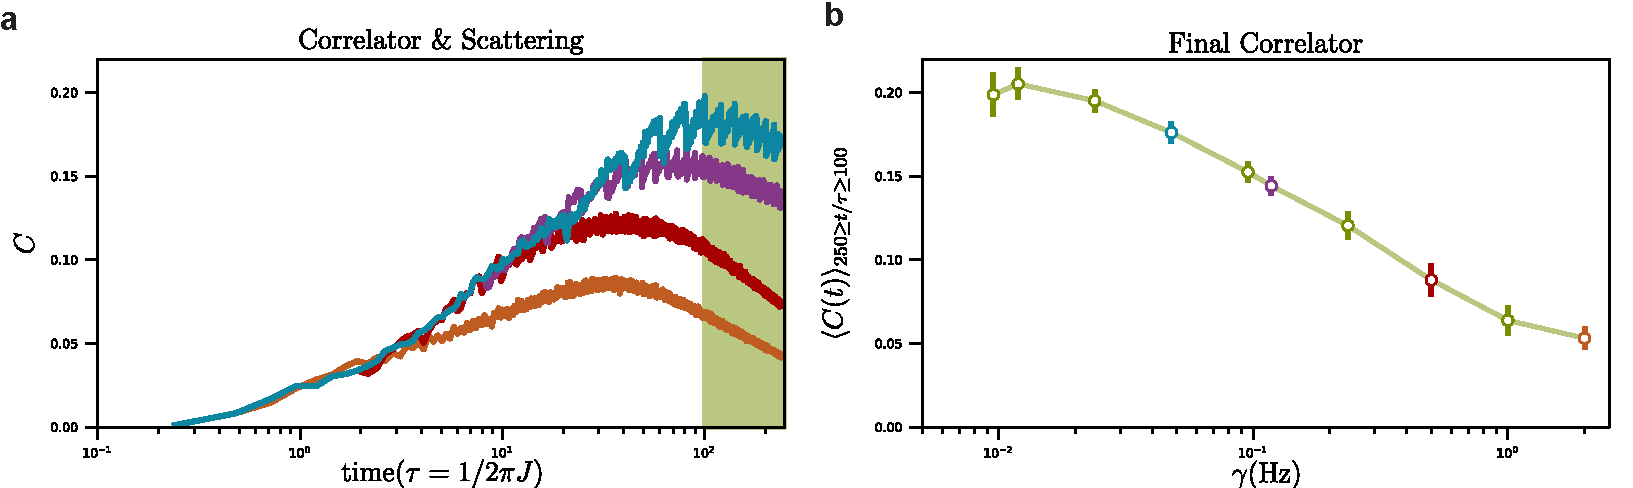
\includegraphics[width=\columnwidth]{figures/ch5/decoherePlot.pdf} 
		\caption{\textbf{Correlator sensitivity to decoherence. a)} The time dynamics of the configurational correlator $C$ when sampled at a periodic rate $\gamma$. The scattering here is modeled to measure the atom-number on a single-site that sees the highest on-site potential offset from the disorder. While the system does not immediately begin to erase the coherences, they are all strongly effected by the final measurement time in our system ($t=100\tau$). \textbf{b)} The averaged correlation value for measurements that happen at a time $100\tau \leq t \leq 250\tau$. This final correlation vale is then plotted as a function of scattering rate in units of the tunneling rate $J$. Note the experimental measured value was $C\approx0.25$. All simulations are calculated by exact diagonalization for the half-size subsystem of a $6$-site Bose-Hubbard chain.}
		\label{fig:MBLgamma}	
\end{figure}

\section{Discussion}

Investigating the growth of non-local quantum correlation has been a long-standing experimental challenge for the study of MBL systems. In addition to achieving exceptional isolation from the classical, external environment and local access to the system, such a measurement requires access to the entanglement entropy \cite{Bardarson2012,Nandkishore2015}. Our work provides a novel technique to characterize the entanglement properties of MBL systems, based on measurements of the particle number fluctuations and their configurations. The observation of slow coherent many-body dynamics along with the breakdown of thermalization allows us to ambiguously identify and characterize the MBL state in our system.

Resolving the genuine growth of correlations related to the logarithmically slow growth of entanglement in the system additionally requires some care in how one averages measurements in the system. Since the configurational correlations, unlike the density-density correlations, are not spatially locked to the underlying correlation of the applied on-site potentials, one has to be careful to always compute $C$ from the quantum average of a given Hamiltonian realization first. Then, the averaging over different disorders realizations can be performed. Otherwise, effectively all configurations will be explored equally among different disorder realizations and the slow entanglement growth will be erased out by the average. This effect does not happen on a qualitative level for the particle number entropy $S_n$ and only changes this observable quantitatively \cite{Lukin2019}.

This distinction in averaging actually provides some additional insight into these correlations as well. In some crude sense, the number fluctuations are a more classical measure that probe thermalization in the system since the eigenstates explore all thermodynamically allowed number states. Then the quantum average over eigenstates and the average over disorders are not particularly different in a qualitative manner. 

Another qualitative way to think about MBL system is that while it does not ergodically explore all number states, it does allow ergodic exploration of the remaining degree of freedom: the configurations of particles restricted to a manifold of local particle number. This, in some sense, sounds like thermalization within a manifold of states where the system can scramble initial phase information\footnote{This refers to the phase information in the superposition of local ``l-bit" creation operators immediately after the quench.} among the remainder of the system. So while the MBL system does not resolve local observables that agree with the global thermodynamic constraints of a thermodynamic ensemble, the system does use a manifold of states as a type of bath for only a subset of states. This additionally implies that while the transport of particles are suppressed in the disordered system, the interactions enable the transport of phase information and has been predicted as a system that enables quantum teleportation of only ``l-bit" phase information.

However, the most fundamental question about this system is whether the transition in behavior of these highly excited eigenstates can be described within the conceptual framework of quantum phase transitions. While this appears as an appealing way to describe the behavior of excited eigenstates, such a relationship has remained elusive due to the difficulty in theory to either compute the behavior of the intermediate disorder regime both numerically or analytically. We will explore such a regime experimentally in an attempt to utilize our quantum simulator to shed some additional light on to this question in the following chapter\cite{Rispoli2018}. 

%PROTECTION OF SYMMETRY AND PHASE TRANSITIONS AMONG MANY EIGENSTATES, CITE HUSE
